\documentclass[12pt,a4paper]{article}

\usepackage[utf8]{inputenc}
\usepackage[english]{babel}
\usepackage{amsmath}
\usepackage{amsfonts}
\usepackage{amssymb}
\usepackage{graphicx}
\usepackage{lmodern}
\usepackage[left=3cm,right=2cm,top=2cm,bottom=2cm]{geometry}
\usepackage{multirow}
\usepackage{booktabs}
\usepackage{array}
\usepackage{tabularx}
\usepackage{amssymb}
\usepackage{here}
\usepackage{tikz}
	\usetikzlibrary{calc}
	\usetikzlibrary{shapes}
	\usetikzlibrary{arrows}
	\usetikzlibrary{fit}
	\usetikzlibrary{positioning}
	\usetikzlibrary{decorations}
	
\begin{document}

\section{Introduction}
Standard workflows in HCI (e.g. user-centered design~\cite{abras2004}) are costly and highly dependent on the person conducting the design process~\cite{liao2021}.
They usually consist of iterative design-evaluate cycles where each step in the design of an artificial system is conducted by a human designer and evaluated by human participants.
Computational HCI (CompHCI)~\cite{oulasvirta2018} is a relatively new research current in HCI which seeks to improve the efficiency of traditional design process by alleviating some of the needs to human resources. It does so by developing mathematical models of users performing tasks, and exploiting these models to drive design and/or decision making of artificial systems.
A core belief driving CompHCI is that many desired designs can be expressed as optimal designs, i.e. one can formulate an appropriate cost function for some family of designs, that, when minimized, will yield the desired design.


CompHCI is an endeavor that requires very different skills and many steps. It will usually include several of the following:
	\begin{itemize}
		\item Building synthetic models of human participants (users) performing particular tasks. Common modeling needs in the interaction context range from low level cognitive models of memory and learning~\cite{nioche2021}, low-level models of motor control~\cite{gori2020} and eye-gaze behavior~\cite{chen2021}, to the high-level mechanisms needed to describe how users perform complex and realistic tasks, that may build off of several low-level models. 

		
		\item Constructing artificial systems that may draw from various computing fields, including and not limited to control theory~\cite{ziebart2012, langerak2020}, machine learning~\cite{koch2019, nioche2021}, optimization~\cite{oulasvirta2020}. 
		
		\item Implementing realistic interfaces that successfully trade-off internal validity with external validity (i.e. interfaces that are both simple and abstract enough that they can be coupled with a synthetic user model, yet complex enough that the results obtained will transpose to real interfaces). 
		
		\item Repeatedly evaluating and calibrating, first synthetic user models, then algorithms, and finally the finished system, potentially with both a synthetic user model and a human user. 

	\end{itemize}


As a result, CompHCI, even more than HCI itself~\cite{blackwell2015}, requires a \emph{collective} effort of researchers that model the user (e.g. behavioral, cognitive, social scientists), that build algorithms (computer scientists, ML researchers, engineering science), that develop interfaces (e.g. designers, web-developers) and that evaluate them (computational scientists, experimentalists). Collective efforts like this are unfortunately difficult; not only is there a ``translation problem'' between different disciplines, researchers from different disciplines also typically pursue different goals~\cite{blackwell2015}, manage different methods and handle different values about what constitutes ``good'' research.




This paper is three things at once. First, it is a call to standardization for research in Computational HCI. We will namely describe what benefits standardization can bring to the multi-disciplinary, collective effort required by CompHCI. 
Second, it is a proposal to use Partially Observable Stochastic Games (POSG) as a common formal model to describe (modern) problems of interest to CompHCI. POSGs are among the most general models that capture the dynamics of interaction of several ---usually two, in case of CompHCI--- agents with (non, partially, of fully) aligned interests. We will explain how POSGs can successfully be used to uniquely describe a large number of interaction scenarios.
Third, it is the presentation of a Python library, called \emph{interaction-agents}, that builds on the POSG model to provide the called-for standard. 
The result is a library with a standardized API, that is modular and favors and re-use of components. It will hopefully allow collective work between independent researchers, in an effort to strengthen the field of CompHCI.


The discussion and presentation throughout this paper will be illustrated by a core problem of HCI that has received much attention, namely pointing facilitation techniques.

\section{Related work}



\subsection{common frameworks, interaction models, Computational HCI}

MPD, POMDP, interventions

TREC Model Harman, D.K., The TREC conferences. Morgan 
Kaufmann Multimedia Information And Systems 
Series247-256. 1997. 


Coadaptation, 


\subsection{Interaction and Artificial Intelligence \label{sub:iui}}
Human decision-making is error-prone, not perfectly rational, variable over time, and humans themselves hold various biases, preferences and goals, all of which, if not accounted for, are potential reasons to explain the failure of an artificial system. Constructing artificial systems that function well when used with/by a human has been a central goal of AI for decades. 


A recent position paper~\cite{dafoe2020}, which introduces the subfield of ``Cooperative AI'' and builds on decades of work conducted in AI, posits that ``machines developed to interact with human partners are more likely to succeed if their design incorporates processes and factors related to human behaviour ---including cognitive heuristics, social cognitive mechanisms, cultural context, legible motion, and personal preferences and expectations''.


Therefore considering how machines can adequately predict the consequences of its actions, predict the other's behavior and account for contributing factors to behavior such as beliefs and preferences is a core requirement for a well performing artificial system~\cite{dafoe2020}.



\subsection{Pointing facilitation}



\section{Call to standardization}
Our call to standardization of CompHCI via an interaction model and an accompanying library is based on the following arguments:
	\begin{itemize}
	\item \textbf{A need for baselines and benchmarks} is acknowledged in most computing fields, and is required for high confidence experiments~\cite{rendle2019}. Benchmarks that are not exceedingly simple have to be uniquely defined rather than approximately replicated by each researcher. Therefore, reliable comparisons and evaluations in CompHCI require some form of task that can be used by various components --- the only way to do so is to build in some form of standard.
	
	\item \textbf{A common conceptual reference} is an asset for researchers who may engage with other colleagues that typically operate in more distant fields. HCI is notoriously interdisciplinary, and even the smaller subset of CompHCI draws on many different computational frameworks. The interaction model that builds on POSGs introduced in this work can serve as a common ground for discussion and reflection. The translation of several different interaction contexts in a formal and abstract framework is likely to enhance collaboration between researchers of different backgrounds, and can hopefully lead to the inclusion of researchers presently external to HCI.
	
	\item \textbf{Re-using and incrementally advancing} prior work by researchers is currently difficult. Owing to the complexity of some of the components involved in CompHCI, we believe working-off of other researchers' work will become more widespread. This re-use is greatly facilitated by having a common way of expressing productions --- such is the case with a common interaction model and a reference API.
	\end{itemize}


We provide some more arguments in favor of each point:




\subsection{Benchmarks}
The idea of having benchmarks and baselines is straightforward: to know how well a production\footnote{We call production any produce of research. In the case of CompHCI, it may be a user model, an interaction technique, an algorithm.} performs, it will be put it in a situation where it can be scored (the benchmark) and compared to some well known competing production (the baseline). The goal for a researcher is to show, objectively and convincingly, that the new production outperforms the baseline on a reference benchmark, and therefore is an advancement to the state of knowledge shared by the community. 

Benchmarks are important catalysts for science; they allow standardized evaluations and therefore indicate which directions are worth pursuing to solve a given problem\footnote{however, caution has to be exerted; the performance-based ``culture to win'' has downsides as well~\cite{lin2019}}. The ImageNet database for example, that is used to benchmark image classification algorithms, is famous for having drawn wide attention to deep learning, when AlexNet significantly outperformed the then best performing algorithms (baseline). 
Baselines and benchmarks are commonly used in HCI. In the domain of pointing facilitation techniques, it is for example common to use a baseline of ``traditional'' pointing on a benchmark known as Fitts' task. This type of comparison is probably the most known and well established in HCI, Fitts' law being a staple of HCI research~\cite{gori2018tochi, soukoreff2004}. Another example is a phrase set for evaluating text entry~\cite{mackenzie2003}. The baseline is usually typing on some reference keyboard.

Fitts' task is likely the least complex benchmark possible in (Comp)HCI; Yet, even this simple benchmark has hard to picture difficulties, see~\cite{guiard2009, gori2018chi}. 
It is not hard to imagine how much more difficult it is to get a more complex benchmark required by CompHCI (see our last argument), such as one needed to realistically simulate some user's task. Therefore, higher validity can be attained if CompHCI researchers use benchmarks that are well established. 


These points are supported by the deep Reinforcement Learning (RL) literature, which handles similarly complex benchmarks (usually called environments). There, the collection of benchmarks known as OpenAI Gym~\cite{brockman2016} has greatly catalyzed the field. It allows objective and fair comparisons between algorithms, which is valuable for established researchers, and also allows newcomers to focus on the learning algorithms, rather than having to deal with implementing an environment first. 
Work in RL also show benchmarks can be hard to get right; there have been many examples of unwarranted behavior emerging from the poor specification of benchmarks (see e.g.~\cite{terry2020, openaicoastrunner}). In particular, some algorithms may learn how to exploit some benchmarks. 


\subsection{Baselines}
Baselines are reference implementations that solve a given problem. They play a very central role in computing fields, namely that of judging whether or not a piece of work improves upon prior work --- which often conditions acceptance. 


There are at least two difficulties with using baselines in (CompHCI). The first, common to most computing fields, is the fact that ``running baselines properly is difficult''~\cite{rendle2019}. In this recent study on recommender systems, it was shown that the baselines that were run by researchers were often much weaker than what is attainable, due to improper hyper-parameter tuning, unwritten ``tricks'' (such as normalizing the data in some phases) and similar practices that are theoretically secondary but which are in practice impactful. A similar observation was reported in the information retrieval community~\cite{lin2019}, where the author suggest authors suffer from confirmation bias: since one's new production is compared against a baseline, there is naturally more incentive to tune one's production than the baseline.
One could argue that the present argument is valid mostly for machine learning algorithms; But machine learning algorithms are being used more and more in (Comp)HCI, and may in some cases become baselines. 

The second difficulty is more related to (Comp)HCI specifically, which, compared to other computing fields, deals with productions that are a lot more high level than algorithms. HCI being an empirical discipline, implementations will matter a lot in the end, and  as a result simple descriptions of systems, such as those typically found in papers, will usually be insufficient to be reproducible. In fact, it can be argued that descriptions of systems are ``always incomplete''~\cite{greiffenhagen2013}, leaving researchers to fill the gaps, and therefore opening an opportunity for suboptimal baselines. 
A solution could be to simply re-use work done by other researchers directly, thereby skipping the re-implementation step. Unfortunately, the high level of productions in HCI means this is again much more difficult, than, say, for an algorithm, see Subs.~\ref{sub:replicate-extend}.

There has been at least one attempt at providing baselines in pointing facilitation technique, by Blanch and Ortega~\cite{blanch2011}, who started a repository of reference implementations of several interaction technique for pointing. While we may not know exactly why it never gained traction, we believe it is at least partly due to the fact that it targeted a very small context of HCI, for which very few pieces of work will be published per year. In contrast, the library we propose targets the broader context of Computational HCI.
 


\subsection{Common Conceptual Reference}
The HCI research landscape has been described as nomadic~\cite{liu2014}, with knowledge that is highly contextual and accumulated around a given technology context (e.g. mouse use). As a result, many researchers frequently embark on new research themes. This is also true of smaller subsets of HCI such as CompHCI.


CompHCI is also a field that draws from many theoretical frameworks. A recently edited collection of works from CompHCI~\cite{oulasvirta2016} lists fields such as control theory, statistical language processing, signal processing, combinatorial optimization and models such as (PO)MDPs, models formulated via differential equations, cognitive architectures used in CompHCI. We can also add usage of information-theory~\cite{gori2020, liu2017, liu2018}, dynamic programming~\cite{jokinen2021, chen2021}, machine learning~\cite{todi2021}. 

Thus, on one hand, (Comp)HCI displays a wide variety of themes of interest, that is also rapidly changing, and on the other hand CompHCI displays a wide variety of theoretical frameworks, as shown by the aforementioned laundry list.
It is without a doubt then, that a structuring, common reference, that formalizes the interaction context into similar components will benefit researchers in CompHCI.
This will notably speed up the learning process necessarily required when jumping from one framework to the other, by providing a common vocabulary and themes that can be reused.


This is particularly true now that research work is increasingly performed in teams~\cite{bennett2013}. This has been shown for virtually all research fields~\cite{wuchty2007}, and it is expected that HCI, and even more so CompHCI, which incorporates many different technical needs, follows as well.



\subsection{Re-use and incrementally advance \label{sub:replicate-extend}}
The acknowledgment of a replication crisis, i.e. the observation that many findings published by a team of researchers could not be reproduced by other independent research teams, has had widespread impact on most fields of science, HCI included. Different voices exist within the HCI community with respect to replication ---what form it should take~\cite{wilson2011}, whether it is needed at all~\cite{greiffenhagen2013}--- likely owing to the diversity of HCI. A model often used in other subfields of computer science is called replicate and extend~\cite{wilson2011}, where work by other researchers is first replicated before being extended with new results or methods. This idea follows from the metaphor of ``standing on the shoulder of giants'', where science advances incrementally. 
While it may be argued that this model may not be suited to HCI at large, once again due to its nomadic nature, it is likely that CompHCI, which handles similar frameworks as other fields of computer science, will benefit from this approach.


Further, we posit that the lack of the replicate and extend approach is at least partially due to the difficulty of actually performing that approach rather than because researchers knowingly choose not to do so.
Usually, systems produced by researchers are prototypes: they are not well maintained, do not support many platforms. Even when the source code is available, porting an entire unknown, usually poorly or entirely undocumented, system to, say, another OS, or a different language, is at best laborious, at worst infeasible.
In all cases, it is extremely unlikely to reliably replicate the system in the first place.
Re-using just parts of the code can be equally difficult; in contrast to an algorithm where the context is perfectly specified by parameters, inputs and outputs, interaction contexts are usually a lot less formally defined, and may include many inter-related code components.






\section{The POSG model as a standard for interaction}
Game theory is typically defined as the study of mathematical models that describe optimal behavior of dynamically interacting agents. A game is a mathematical object, which describes how agents will observe the situation, and how they will perform actions.

Perhaps surprisingly, the HCI and game theoretic literature, which thus both primarily deal with interaction, have very little overlap. In this section, we show that interaction can be modeled as a game in the game-theoretic sense, namely as a Partially Observable Stochastic Game (POSG).
\subsection{Partially Observable Stochastic Games}
A partially observable stochastic game (POSG) is a tuple $(\mathcal{I}, \mathcal{S}, \lbrace \mathcal{A}_i \rbrace, \lbrace \mathcal{O}_i \rbrace, \mathcal{P}, \lbrace R_i \rbrace )$, where $\mathcal{I}$ is the finite set of agents indexed by $i \in [1,\dots,n]$, $\mathcal{S}$ is the set of states, $\mathcal{A}_i$ is the action set for agent $i$. $\mathcal{A}$ is the joint action set $(\times_{i} \mathcal{A}_i)$ for all agents, and the joint action is $a = (a_1, \dots{}, a_n)$, $\mathcal{O}_i$  is the observation set for agent $i$. A joint observation is $o=(o_1, \dots{}, o_n) \in \times_i \mathcal{O}_i$. $\mathcal{P}$ is a state transition and observation probability: $P(s', o| s, a)$ is the probability of the state transitioning from $s$ to $s'$ and the agent observing $o$ after they have taken the joint action $a$ in state $s$.
Finally, $R_i(s,a)$ is the reward for agent $i$, after the joint action $a$ was taken in state $s$.
In a POSG, all agents simultaneously select an action, receive a reward, and observation. The goal of each agent is to maximize its sum of rewards over the course of the many interactions it will have with the game. 




\subsection{A user-assistant model of interaction}
A user-assistant model can be successfully used in contexts where a user interacts with an interface to complete a task, and serves as a stepping stone towards modeling interactive settings via POSGs. It assumes that there is a \textbf{task} which can be fully represented by a state \(s_T\), that there is a \textbf{user} who wants to drive the task to a goal state, and has some fixed set of actions to do so, and that there is some component to the interface that is capable of taking actions with regards to the current state or history of states of the task and/or the user to \textbf{assist} the user in attaining its goal.


\paragraph{Agents.} Both the user and assistant are agents in the game-theoretic sense, and posess the following properties, in line with Subs.~\ref{sub:iui}
\begin{itemize}
\item They have an internal state ($s_O$ and $s_A$ for respectively the user and the assistant) which stores e.g. goals, preferences, model parameters ---virtually anything that is susceptible of varying over time.
\item They have the ability to observe (perfectly or partially) the various states of the components of the interaction model. When making an observation ($o_O$ and $o_A$), the agents may receive a reward, to account for the fact that they could perceive a cost (e.g. because that observation may take some time to be created) or a benefit (e.g. because it satisfies a curiosity) to making an observation.
\item Based on these observations, they are able to make inferences that change their internal states. The agents may again here receive a reward, since there could be a cost to inferring (e.g. mental effort, computational resources) or a benefit (e.g. satisfaction).
\item Based on their internal states and their observations, they are able to take actions ($a_O$ and $a_A$) via a policy. Those actions may have an effect on the other states of the interaction model.
\end{itemize}

\paragraph{Rounds and turns.} A round of interaction is played in four turns, and is defined by the following sequence of events :
$$s^{(0)} \rightarrow o'_U \rightarrow s^{(1)} \rightarrow a'_U \rightarrow s^{(2)} \rightarrow o'_A \rightarrow s^{(3)} \rightarrow a'_A \rightarrow s^{'(0)},$$
where $s^{(k)}$ is the joint state formed by the turn number $k$, and the states of the task, the user and the assistant:
\[\begin{split}s^{(0)} = (0, s_T, s_U, s_A), \\ s^{(1)} = (1, s_T, s'_U, s_A), \\ s^{(2)} = (2, s'_T, s'_U, s_A), \\ s^{(3)} = (3, s'_T, s'_U, s'_A), \\ s^{'(0)} = (0, s''_T, s'_U, s'_A).\end{split}\].

In plain language, a turn starts at some specific joint state. The user then observes the joint state; based on that observation, it updates its internal state (turn 1). It then takes an action (turn 2). Turns 3 and 4 are equivalents with the assistant. 


\paragraph{Rewards} At each turn, rewards are issued, either by the state, the user or the assistant. The need for rewards is directly linked to the core idea of optimal designs that is central to CompHCI.


The relationship between agents, turns and rewards is recapitulated in Fig~\ref{fig:sequence_events}.

\begin{figure}
\centering
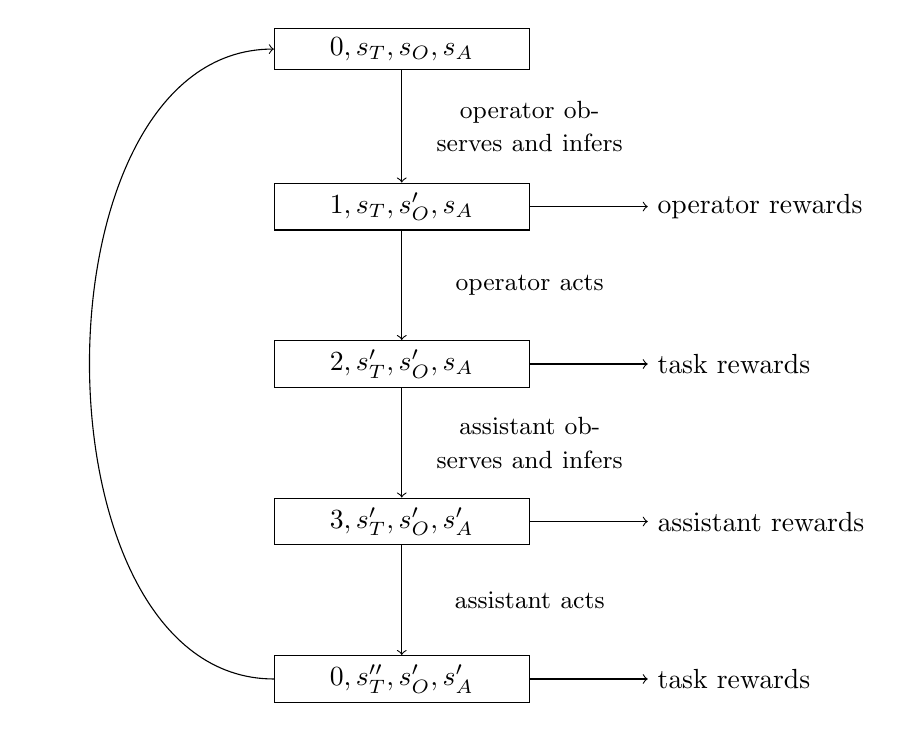
\begin{tikzpicture}
\draw (0,0) node[rectangle, draw = black, name = s0, text width = 3cm, text centered]{$0,s_T, s_O, s_A$};
\draw (s0) + (0,-2) node[rectangle, draw = black, name = s1, text width = 3cm, text centered]{$1,s_T, s'_O, s_A$};
\draw[->] (s0) -- node[midway, right, text width = 3cm, text centered]{\small operator observes and infers} (s1);
\draw[->] (s1.0) -- + (1.5,0) node[right]{operator rewards};
\draw (s1) + (0,-2) node[rectangle, draw = black, name = s2, text width = 3cm, text centered]{$2,s'_T, s'_O, s_A$};
\draw[->] (s1) -- node[midway, right, text width = 3cm, text centered]{\small operator acts} (s2);
\draw[->] (s2.0) -- + (1.5,0) node[right]{task rewards};
\draw (s2) + (0,-2) node[rectangle, draw = black, name = s3, text width = 3cm, text centered]{$3,s'_T, s'_O, s'_A$};
\draw[->] (s2) -- node[midway, right, text width = 3cm, text centered]{\small assistant observes and infers} (s3);
\draw[->] (s3.0) -- + (1.5,0) node[right]{assistant rewards};
\draw (s3) + (0,-2) node[rectangle, draw = black, name = s4, text width = 3cm, text centered]{$0,s''_T, s'_O, s'_A$};
\draw[->] (s3) -- node[midway, right, text width = 3cm, text centered]{\small assistant acts} (s4);
\draw[->] (s4.0) -- + (1.5,0) node[right]{task rewards};
\draw[->] (s4.180) to[out=180, in=180] (s0.180);
\end{tikzpicture}
\caption{Order of events in a round of interaction. \label{fig:sequence_events}}
\end{figure}


\subsection{Relation to POSG}
For different turns, we define the following joint observations
$$ o^{(1)} = (o'_O, \text{No-Op}), \quad o^{(2)} = (\text{No-Op}, \text{No-Op}), \quad o^{(3)} = (\text{No-Op}, o'_A), \quad o^{'(0)} = (\text{No-Op}, \text{No-Op})$$
and joint actions:
$$a^{(0)} = (\text{No-Op}, \text{No-Op}),\quad a^{(1)} = (a'_O, \text{No-Op}),\quad a^{(2)} = (\text{No-Op}, \text{No-Op}),\quad a^{(3)} = (\text{No-Op}, a'_A),$$
where No-Op is a so-called No-Operation flag, which signals that the component is void.
The user-assistant model can be modeled by a POSG, with the following transition and observation probabilities:

\[\begin{split}p(s^{(1)}, o^{(1)} | s^{(0)}, a^{(0)}) & = p(o^{(1)} | s^{(0)}, a^{(0)}) \cdot{} p(s^{(1)}| o^{(1)}, s^{(0)}, a^{(0)}) \\ &= \underbrace{p(o'_O | s^{(0)})}_\text{user observation function } \underbrace{p(s^{(1)}| o'_O, s^{(0)})}_\text{ user inference function} \\ p(s^{(2)}, o^{(2)} | s^{(1)}, a^{(1)}) & = p(s^{(2)}| s^{(1)}, a^{(1)}) \\ &= \underbrace{p(s^{(2)}| s^{(1)}, a'_O)}_\text{ user step function} \\ p(s^{(3)}, o^{(3)} | s^{(2)}, a^{(2)}) & = p(o^{(3)} | s^{(2)}, a^{(2)}) \cdot{} p(s^{(3)}| o^{(3)}, s^{(2)}, a^{(2)}) \\ &= \underbrace{p(o'_A | s^{(2)})}_\text{assistant observation function } \underbrace{p(s^{(3)}| o'_A, s^{(2)})}_\text{ assistant inference function} \\ p(s^{'(0)}, o^{'(0)} | s^{(3)}, a^{(3)}) & = p(s^{'(0)}| s^{(3)}, a^{(3)}) \\ &= \underbrace{p(s^{'(0)}| s^{(3)}, a'_A)}_\text{ assistant step function} \\\end{split}\]

The transition and observation probabilities of the POSG can therefore be described by a different function for each turn of the game, which in turn can be separated again into an \textbf{observation function}, an \textbf{inference function} and a \textbf{step function}, each for the user and the assistant. These functions will form the basis of the library's structure.

   

\subsection{Pointing Facilitation Example}
We gave no proof that interactive contexts common in (CompHCI) could be represented by a user-assistant model and thus as POSGs
\footnote{This would likely be impossible anyway since there is no formal definition for what an interactive context in HCI is; in fact, it is what we are trying to define in this paper in the first place.}. Instead we show how a simple pointing facilitation technique can be expressed as a POSG, as an illustrative example, representative of many other interaction techniques and interactive contexts.  


In experiments involving pointing facilitation techniques, the task is usually for the user to select a given target among $n$ potential targets, via mouse input.
Let us consider a simple toy pointing task, formulated as a 1D gridworld:
\begin{figure}[H]
\begin{verbatim}
       |P| | | | | |T| | | | | | | | |G| | |T| | | | | | |T| | | | | |
\end{verbatim}
\caption{A gridworld example for pointing}
\end{figure}

\noindent where \texttt{P} is the current position of the cursor, \texttt{G} is the (fixed) position of the goal the user is trying to reach and the \texttt{T}'s are the (fixed) positions of targets on the grid.
\textbf{The task} is fully defined by its state, $S_T = \lbrace P, \lbrace T_i \rbrace_{i=1}^n \rbrace$, i.e. the current position of the cursor and targets. The \textbf{user}'s state $S_U = \lbrace G \rbrace$ consists of the goal target \texttt{G}. In a more complex example, it could also hold parameter values that relate to preferences, biases etc. as discussed in Sub.~\ref{sub:iui}. The \textbf{assistant} here will be a replication of BIGPoint, introduced as a tutorial method in~\cite{lui2017} for the more complex BIGNav. It maintains a belief state $S_A = \lbrace \lbrace p(T_i) \rbrace_{i=1}^n \rbrace$, where each $p(T_i)$ maps a target to a probability (it represents how much the assistant believes a particular target may be the user's goal).





The goal of the operator is to move the cursor to the goal \texttt{G}. To do so, he can produce an action $a_1 \in \mathcal{A}_1 =  \lbrace -N, -N +1, \dots{}, -m -1, -m, \dots{} m, m+1, \dots{} N-1, N \rbrace$. If $\mathcal{A}_1 = \lbrace-6, -5, -4, -3, -2, 2, 3, 4, 5, 6 \rbrace$, the operator is able to move to any place between 2 and 6 units away in both directions. 


The goal of the enhancer is to assist the operator in selecting his goal. To do so, he can produce an action $a_2 \in \mathcal{A}_2 = [0,K]$ (assume $K=5$), that will modulate the operator's action. If we denote $P(t)$ the position at timestep $t$, then the modulation has the following form:
\begin{align}
P(t+1) = P(t) + \Delta t \label{eq:toy_problem_model_1} \\
\Delta t =  a_1 \times (1 + a_1 \varepsilon) \times a_2, \label{eq:toy_problem_model_2}
\end{align}
\noindent where $\varepsilon \sim  \mathcal{N}(0,1)$. The term $a_1 \varepsilon$ represents signal dependent noise, i.e. the fact that in many real-world scenarios the noise in operator's actions increases with that actions' amplitude.
Although this model appears to be quite simple, it captures many interesting properties of the transfer function context:

\begin{itemize}
\item The action space of the operator is bounded. In this simple model, it has a minimum traveling distance ($|m|=2$), and a maximum traveling distance ($|M| = 6$). This captures the limitations that there is a minimum and maximum speed achievable when operating a mouse.
\item The noise associated with the operator's action is signal dependent, i.e. noise increases with the signal value. This is characteristic of human produced movement.
\item The enhancer's action is a simple gain applied to the operator's action, as is the case with transfer functions.
\end{itemize}

Why would the operator need gain ? Well for once, the enhancer allows the operator to go past it bounds, by increasing the maximum distance that can be traveled as well as decreasing the minimum distance that can be traveled. The range that is effectively attainable in one step is now (supposing noiseless case) $[0;30]$.
A second reason is because of noise: To move 6 units to the right, the following two couples will do 
	
\begin{itemize}
	\item No enhancer action: $(a_1 = 6, a_2 = 1)$, in which case $\Delta t = 6 + 36 \varepsilon$
	\item Smallest operator action: $(a_1 = 2, a_2 = 3)$, in which case $\Delta t = 6 + 6\varepsilon$
\end{itemize}		
\noindent So, an other advantage provided by the enhancer is that it will lead to less propagation of noise.

\section{}

exploits various computational techniques and tools (control theory, information theory, optimization), 





One of the promises of CHCI is to make use of computational methods to achieve optimal\footnote{By optimal, we mean that the final design is the one that maximizes some score that has been chosen by the designer. While this may not be a holistic approach, it has the benefit of making the design problem amenable to formal methods, and thus automatable, as well as removing potential subjective interpretations and biases during the design process. Nothing prevents to use computational methods in complement to other more classical methods.} designs.


While there is no standard workflow in CHCI, the principles advocated by CHCI requires one to
\begin{description}
\item[Develop user models.] These are required to describe human behavior in terms usable by algorithms, which use them to form predictions of the effectiveness of potential decisions~\cite{oulasvirta2021}. For example, a user model of item selection time in a menu was leveraged in~\cite{todi2021} to help build adaptive menus. Another example is given by the BIG framework~\cite{liu2017, liu2018}, where an algorithm maximizing Expected Information Gain requires the probabilities with which the user will produce any action in any situation.


Models needed in HCI can target low-level psychological mechanisms, such as motor control~\cite{gori2020}, visual search~\cite{acharya2017}, foveal vision~\cite{chen2021}, reaction times~\cite{liu2020}, or higher-level complex mechanisms which describe complete task completions e.g. touch-typing~\cite{jokinen2021}. These higher-level mechanisms can partially be formed by the combination of several low-level mechanisms (for example the touch-typing model combines low level models of pointing, vision and proofreading).


Models can be expressed as mathematical functions (e.g. neural nets, likelihoods), frequency tables, rules.

\item[Develop artificial systems.] These are the actual systems of interest to HCI. These make use of various objective criterion to assess the goodness of the system and various algorithms to reach those objectives.

One difficulty here is that there are very limited standard implementations artificial systems
\begin{itemize}
\item Usually, systems are too complex to describe in a paper. Similarly, there is no culture of accurately describing algorithms such that they are replicable in HCI.
\item While systems may be released, they are usually much more complex than a couple functions, and they are written in some specific language. This makes it hard for an independent researcher to use the system inside its own framework e.g. to use as baseline.
\end{itemize}


\item[Simulate/Evaluate.] Simulations can be used to assess whether the couple (simulated user, artificial system) works as intended. Simulations can also be the primary decision-making means for certain algorithms.
When developing artificial systems based on computational interaction, one will leverage a computing language (e.g. Python) during initial phases when producing simulations, but the final system to be evaluated with a user may often implemented in a language more suited to building interfaces.
\end{description}

Research in CHCI today lacks the discipline that is expected from scientific research, in particular, it is very hard for a researcher to build on another researcher's work, e.g. in an effort to provide an incremental enhancement to one's work, to use as a baseline, or to re-use a component that was successful in doing something.


Second, engaging in CHCI requires to have knowledge in
	\begin{itemize}
		\item Model building, model evaluation. usually done by cognitive scientists that work at the interface with HCI.
		\item Constructing artificial systems, which usually consists in recuperating algorithms from fields such as computer science, AI, and re-using them, with or without adaptation.
		\item Implementing realistic interfaces, in which users can engage with the artificial system for evaluation.
	\end{itemize}

These three items require vastly different skills, and it is expected that many research projects engaging in CHCI, even when the research team may be compromised of researchers of varying profiles, will compromise on at least one aspect of it.
It would therefore be tremendously helpful if different people from different teams could cooperate. e.g. Team 1 builds a model, Team 2 implements a new smart assistant. Team 3 takes care of getting data from a real interface and makes it amenable to changes.

The goal of this library is to improve the state of CHCI research, by ``treating'' the problems above.
We do so by:
	\begin{itemize}
	\item Providing a common interface for objects so that components may be re-used (including a registration of components)
	\item allowing modularity by building high level models from low level components
	\item allowing a bridge between Python and any other language supporting websockets, thereby allowing one to code the interface in some language, and have the computational modeling done via Python.
	\end{itemize}



\newpage



\newcolumntype{r}{>{\bfseries}l}
\begin{table}[ht]
\centering%
\resizebox{\textwidth}{!}{
\begin{tabular}{lcccccc}
    & & \textbf{Working now} & \textbf{Step 1} & \textbf{Step 2} & \textbf{Step 3} & \textbf{Final Setup}  \\
    \toprule
    \multirow{2}{*}{\textbf{Evaluation}}& Synthetic User Model & \checkmark & \checkmark & \checkmark &  & \checkmark \\
    & Real User &  &  & & \checkmark & \checkmark  \\
    \cmidrule{2-7}
    \multirow{2}{*}{\textbf{Task}}& Abstract Task & \checkmark & \checkmark & \checkmark & & \checkmark\\
    & Realistic Task &  & & & \checkmark &  \checkmark \\
    \cmidrule{2-7}
    \multirow{4}{*}{\textbf{Assistance}}& User Agnostic  & \checkmark & \checkmark & \checkmark & \checkmark & \checkmark \\
    & User Model Given & \checkmark & \checkmark & \checkmark & \checkmark & \checkmark \\ & User Model Structure Given, parameters learned &  & \checkmark & \checkmark & \checkmark & \checkmark \\ & User-gnostic, nothing given & & \checkmark & \checkmark  & \checkmark & \checkmark \\
    \cmidrule{2-7}
   	 \multirow{3}{*}{\textbf{User Model}}& Explicit likelihood-based model & \checkmark & \checkmark & \checkmark &  --- &  \checkmark \\
    & trained/tuned user model & \checkmark & \checkmark & \checkmark & --- &  \checkmark \\ & Nested simulation models & \checkmark & \checkmark & \checkmark & --- &  \checkmark \\
    \cmidrule{2-7}
     \multirow{2}{*}{\textbf{Adaptivity}}& Static policies & \checkmark & \checkmark & & & \checkmark \\
     & Adaptive Assistance with adaptive user policy &  & & \checkmark & \checkmark & \checkmark \\
    \bottomrule
\end{tabular}
}
\end{table}

\newpage

\section{quotes}



 
 



While CompHCI does not yet provide user models complex enough to simulate user behavior on a real software interface, there have been some recent examples of higher level tasks, such as single-finger touch-typing with proofreading~\cite{jokinen2021}.
\end{document}